\begin{enumerate}
	\item Exercício retirado da página 1023 de \cite{James_Stewart_calculo_v2}
	
	Calcule $$\iiint_E \sqrt{x^2 + y^2 + z^2}\, dv$$, onde $E$ é limitado abaixo pelo cone $\phi = \dfrac{\pi}{6}$ e acima pela esfera $\rho = 2$.
	
	\begin{figure}[htb]
		\caption{Coordenadas esféricas - Aula 07 - Exercício I}
		\label{v24_a07_e01}
		\centering
		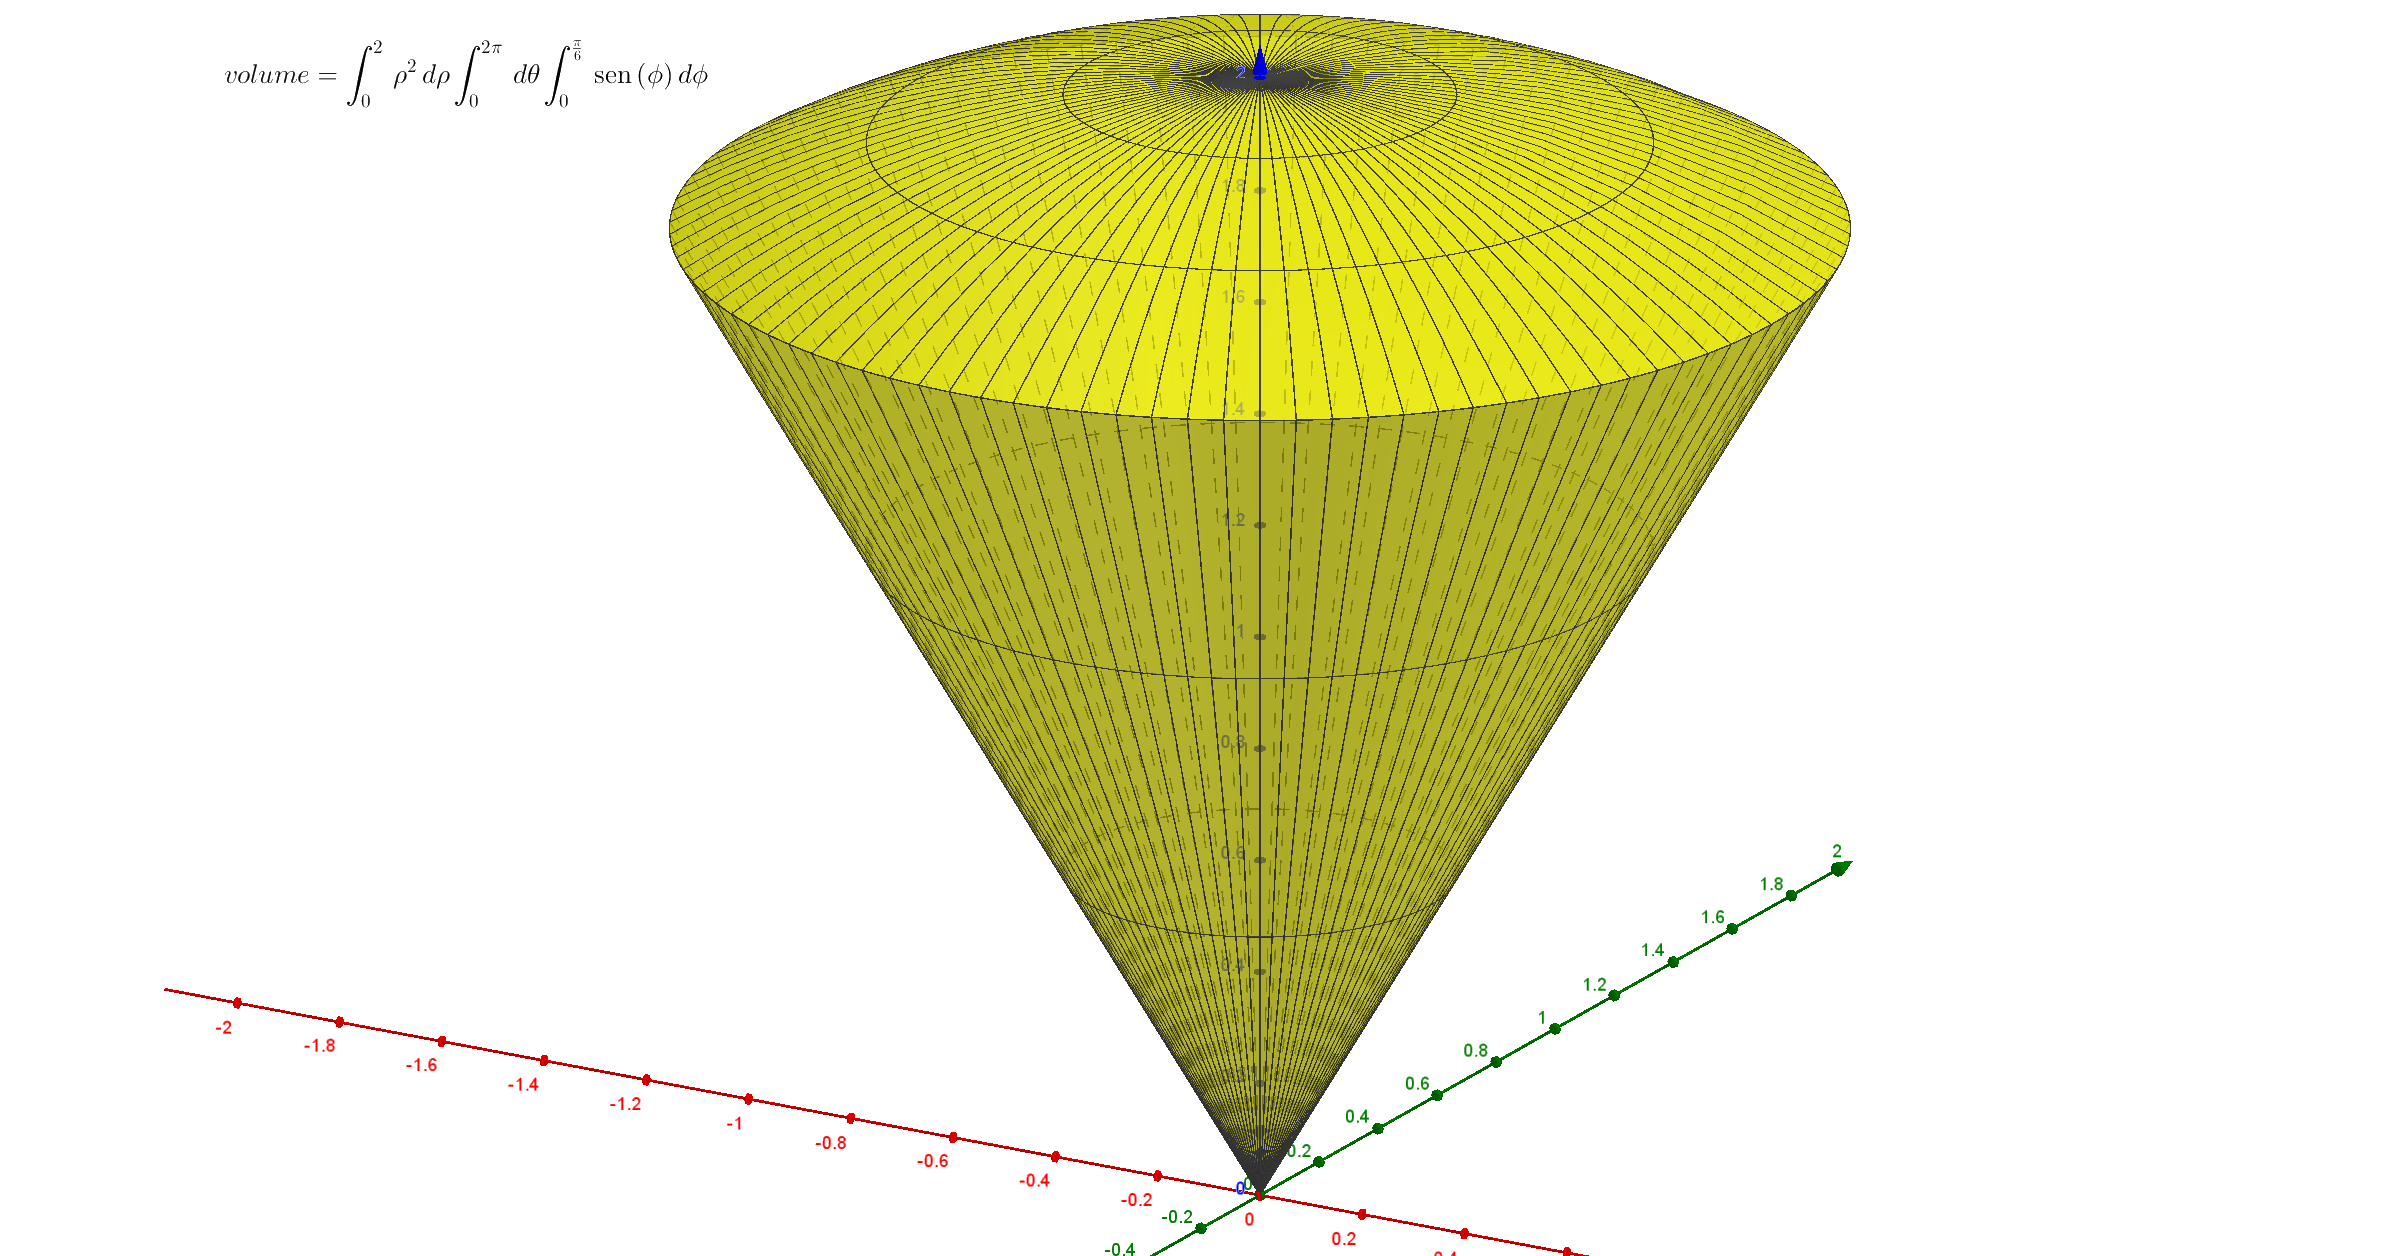
\includegraphics[width=0.5\textwidth]{v24_a07_e01.png}		
	\end{figure}
	
	\begin{equation*}
		0 \leq \rho \leq 2,\, 0 \leq \theta \leq 2\pi,\, 0 \leq \phi \leq \dfrac{\pi}{6}
	\end{equation*}
	\begin{equation*}
		\sqrt{x^2 + y^2 + z^2} = \sqrt{\rho^2} = \rho
	\end{equation*}
	\begin{equation*}
		dv = \rho^2\sen(\phi)\, d\rho d\theta d\phi
	\end{equation*}
	\begin{gather*}
		\iiint_E \sqrt{x^2 + y^2 + z^2}\, dv = \int_0^2 \int_0^{2\pi} \int_0^{\frac{\pi}{6}}(\rho)\rho^2\sen(\phi)\, d\phi d\theta d\rho =\\ \int_0^2\rho^3\, d\rho \int_0^{2\pi} d\theta \int_0^{\frac{\pi}{6}}\sen(\phi)\, d\phi = \left[\dfrac{\rho^4}{4}\right]_0^2 \left[\theta\right]_0^{2\pi} \left[-\cos(\phi)\right]_0^{\frac{\pi}{6}} =\\ \dfrac{16}{4}2\pi\left(-\cos\left(\dfrac{\pi}{6}\right) + \cos(0)\right) = 8\pi\left(\dfrac{-\sqrt{3}}{2} +  1\right) = 8\pi \dfrac{-\sqrt{3} + 2}{2} = 4\pi\left(2 - \sqrt{3}\right)
	\end{gather*}
\end{enumerate}